\subsection*{\textbf{Question 1.d)}}
\begin{quote}

\textbf{Problem}
\begin{quote}
Write a code that does the Kuiper’s test on your random numbers (see tutorial
8) and make the same plot as for the KS-test.
\end{quote}

\textbf{Solution} 
\begin{quote}
The implementation of the Kuiper test does require a numerical approximation of the CDF for the kuiper statistics. The CDF of the kuiper staistic is given by, 
\begin{equation}
P_{kuiper}( \lambda) =  1 - 2  \sum_{j=1}^{\infty} (4j^2 \lambda^2-1) e^{-2j^2 \lambda^2 }
\end{equation}

The sum is in the above expression negligible compared to the machine error if $\lambda < 0.4$. In this case the numerically approximation thus consist of returning 1.  If $\lambda > 0.4$ then the sum is approximated by calculating the first 100 terms of the sum. This should be more than enough for the sum to converge. \footnote{In theory less terms are enough. The evaluation of the sum could therefore stop early by checking for a required precision. } 

The kuiper test and the CDF are implemented in the shared module \texttt{./Code/mathlib/statistics.py} on page \pageref{CODE:Statistics}. The code that creates the plots and the plots can be found below.  The code does make use of \textbf{astropy} to compare the self written implementation of the Kuiper-test with the implementation of astropy. 
\end{quote}

\textbf{Code - Plots}

\begin{quote}
The code for generating the two plots. The imports are not explicit shown but can be shown on page \pageref{CODE:MAIN1}. 
\lstinputlisting[firstline=183,lastline=236]{./Code/assigment_1.py}
\end{quote}

\textbf{Code - Output plot(s)}
\begin{quote}
\begin{figure}[!ht]
\centering
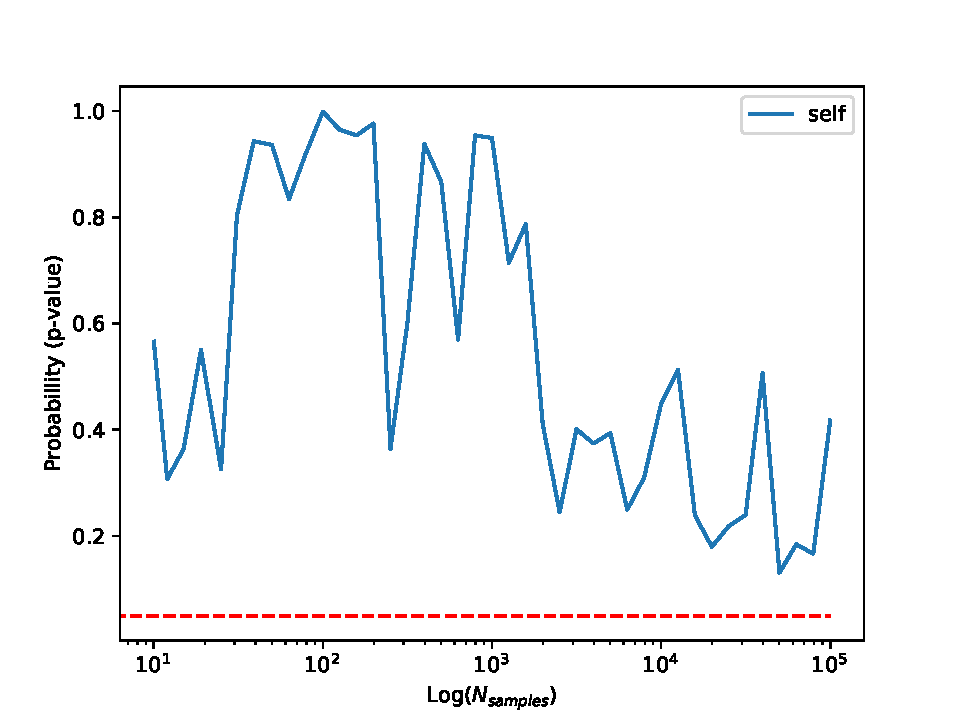
\includegraphics[width=12cm, height=7.5cm]{./Plots/1_plot_kuiper_test_self.pdf}
\caption{The P-value produced by the kuiper test against the number of samples on which the kuiper-test is performed for the self written RNG. The red line indicates the line of $ p = 0.05$. A point \textbf{below} there  line would suggests that there is enough statistical evidence to reject the (null) hypothesis that the data is normal distributed. The plot shows that the RNG always passes kuiper test. It can however be seen that the p-value stays lower for larger sample size, similar as with the KS-test.}
\end{figure}
\newpage
\begin{figure}[!hb]
\centering
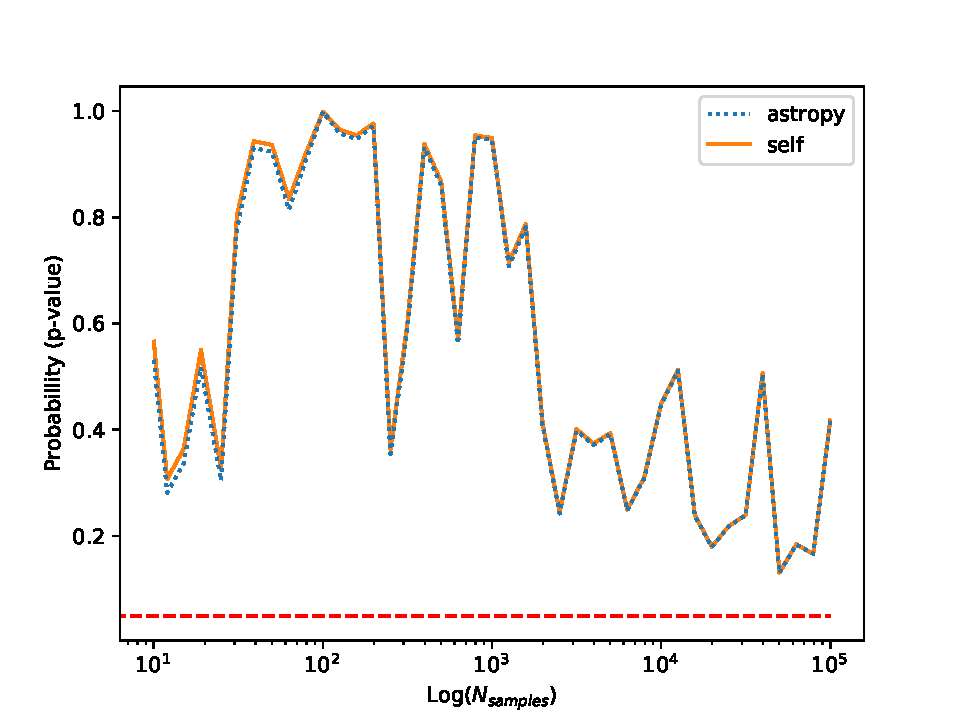
\includegraphics[width=12cm, height=7.5cm]{./Plots/1_plot_kuiper_test_self_astropy.pdf}
\caption{The P-value produced by the kuiper test against the number of samples on which the kuiper-test is performed for the self written RNG. The red line indicates the line of $ p = 0.05$. A point \textbf{below} there  line would suggests that there is enough statistical evidence to reject the (null) hypothesis that the data is normal distributed. The plot shows that the self written implementation has (small) deviations from the astropy implementation at small sample sizes. This is similar to the situation with the KS-test and might be caused by an approximation made in astropy.   }
\end{figure}

\end{quote}
\end{quote}














